\documentclass[12pt,a4paper]{cv}

\begin{document}

%--------------------------------------------------
% HEADING
%--------------------------------------------------
\parbox{25mm}{%
	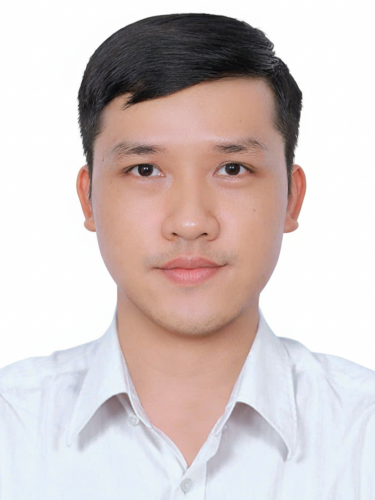
\includegraphics[width=2.35cm,clip]{avt.png}
}
\parbox{\dimexpr\linewidth-25mm}{
	\begin{tabularx}{\linewidth}{X r}
		\cvName{Thinh}{Nguyen Phuoc} & \\
		\textit{Software Engineer} & (+84)989 098 494 \\
		& September 26, 1996 \\
		& \href{mailto:npthinh1996@gmail.com}{npthinh1996@gmail.com} \\
		Tan Hoa Ward & \href{https://www.linkedin.com/in/thinh9e/}{linkedin.com/in/thinh9e} \\
		Ho Chi Minh City, VN & \href{https://thinhblog.com}{thinhblog.com}
	\end{tabularx}
}
\medskip
\\
Software Engineer with over 5 years of experience developing high-performing applications in Agile environments. Experienced in optimizing databases, enhancing security, and collaborating to deliver impactful results. Skilled at leveraging AI tools to boost development productivity.
\bigskip


%--------------------------------------------------
% EDUCATION
%--------------------------------------------------
\begin{cvSection}{Education}

	\textbf{Ho Chi Minh City University of Technology (HCMUT)} \hfill \textit{Sep 2014 -- Nov 2019} \\
	B.S. in Computer Science \& Engineering \\
	GPA: 7.42/10

\end{cvSection}


%--------------------------------------------------
% WORK EXPERIENCE
%--------------------------------------------------
\begin{cvSection}{Work Experience}

	\begin{cvSubsection}{FPT Software}{Mar 2025 -- Present}{Software Engineer}
		\item Contributed to the Automotive project for a US customer.
		\item Enhanced and optimized Python code within AWS Lambda functions.
		\item Improved code quality by implementing component tests.
		\item Migrated AWS services and REST API endpoints.
		\item Leveraged AI tools to improve development productivity.
	\end{cvSubsection}

%--------------------------------------------------

	\begin{cvSubsection}{TMA Solutions}{Mar 2019 -- Mar 2025}{Software Engineer}
		\item Contributed to the Network Performance Monitoring project for a US customer.
		\item Collaborated on new features, improving UX/UI, and system functionality.
		\item Optimized query execution times to enhance application performance.
		\item Troubleshot and resolved critical customer issues.
		\item Identified and mitigated security vulnerabilities to prevent potential breaches.
		\item Managed lab servers and implemented performance systems.
	\end{cvSubsection}

%--------------------------------------------------

	\begin{cvSubsection}{MangoAds}{Jun 2018 -- Aug 2018}{Intern}
		\item Automated content collection and import for WordPress pages.
		\item Developed a web application to track keyword rankings on major search engines.
		\item Continuously enhanced skills through online courses.
	\end{cvSubsection}

\end{cvSection}


%--------------------------------------------------
% SKILL
%--------------------------------------------------
\begin{cvSection}{Skill}

	\begin{tabular}{@{} >{\bfseries}l @{\hspace{6ex}} l @{}}
		Languages & Python, Java, C/C++ \\
		Frameworks & Django, Spring, Bootstrap \\
		Databases & MariaDB, SQL Server \\
		Cloud & AWS \\
		Tools & Git, SVN, Docker, IntelliJ, VSCode, Burp Suite \\
		AI & Copilot, Ollama, Rasa, LangChain \\
	\end{tabular}

\end{cvSection}


%--------------------------------------------------
% PROJECT
%--------------------------------------------------
\begin{cvSection}{Project}

	\begin{cvSubsection}{Web Checker}{Dec 2018 -- Present}{
			Project URL: \cvLinkURL{https://github.com/thinh9e/web-checker}
		}
		\item Developed a Django web application to evaluate SEO scores using the MVC pattern.
		\item Implemented content retrieval, parsing, and link status to identify and generate scores.
		\item Utilized thread pool for concurrent request handling, significantly reducing response time.
	\end{cvSubsection}

%--------------------------------------------------

	\begin{cvSubsection}{Centralized Synchronization Services}{Mar 2024 -- Mar 2025}{}
		\item Collaborated with the team to design and implement the system architecture.
		\item Implemented Spring Integration to manage distributed services via a message queue.
		\item Implemented Server-Sent Events for communication between services.
		\item Optimized resource utilization by applying Java virtual threads to the thread pools.
	\end{cvSubsection}

%--------------------------------------------------

	\begin{cvSubsection}{Burp Suite Automation}{Aug 2021 -- Jun 2023}{}
		\item Developed a tool that integrates with Burp Suite through a custom proxy.
		\item Built with Selenium for web browser automation and Tkinter for an interactive GUI.
		\item Deployed the tool to enhance automated security scanning within our project workflows.
	\end{cvSubsection}

%--------------------------------------------------

	\begin{cvSubsection}{Checksum Generator}{Dec 2021 -- Dec 2021}{}
		\item Developed a pure Python checksum generation tool to ensure data integrity.
		\item Implemented JSON configuration to track file status changes (add/modify/delete).
		\item Integrated the tool into the project, ensuring seamless operation in customer deliverables.
	\end{cvSubsection}

\end{cvSection}


%--------------------------------------------------
% CERTIFICATE
%--------------------------------------------------
\begin{cvSection}{Certificate}

	\begin{cvSubsection}{AWS Essential Training for Developers}{Aug 2025}{
			LinkedIn Learning: \cvLinkURLText{https://www.linkedin.com/learning/certificates/49f19f734a33d78bde62ae4d938768a0d6c4c255813babc17365f9a84427707a}{Show credential}
		}
		\item[] Learned how to build and deploy applications on AWS.
	\end{cvSubsection}

%--------------------------------------------------

	\begin{cvSubsection}{Learning How to Learn}{May 2025}{
			Coursera: \cvLinkURLText{https://www.coursera.org/account/accomplishments/verify/P85UPP9ZC738/}{Show credential}
		}
		\item[] Learned how the brain learns to help master any subject.
	\end{cvSubsection}

%--------------------------------------------------

	\begin{cvSubsection}{Intermediate to Advanced Python with 10 OOP Projects}{Jan 2024}{
			Udemy: \cvLinkURLText{https://ude.my/UC-31536a7e-1d52-4cb2-b73d-60bbe5525a33/}{Show credential}
		}
		\item[] Learned Python in OOP, Git, APIs, databases, deployment, PEP8, and more.
	\end{cvSubsection}

\end{cvSection}


%--------------------------------------------------
% AWARD
%--------------------------------------------------
\begin{cvSection}{Award}

	\begin{cvSubsection}{AI Contest 2023}{Oct 2023}{TMA Solutions -- DG}
		\item Placed third in an AI contest.
		\item Developed an AI chatbot that seamlessly integrates with customer systems.
		\item Engineered to answer FAQs and interact with system services via a REST API.
	\end{cvSubsection}

\end{cvSection}

\end{document}
